\section{Question 1: Representation Learning in Text Classification}

\subsection{Dataset Description}

Question 1 uses the IMDb movie-review sentiment benchmark \cite{maas2011imdb}, which contains 50{,}000 balanced reviews split into 25{,}000 original training examples and 25{,}000 original test examples. In the final full-data run used here, the original training split is divided into 20{,}000 training and 5{,}000 validation examples, while the full 25{,}000-example IMDb test split is kept for final evaluation. Because the labels are exactly balanced, accuracy and macro-F1 move closely together and give a stable summary of comparative performance.

\subsection{Preprocessing Pipeline}

All Q1 models share the same base text-normalization pipeline: HTML tags are stripped, text is lowercased, non-alphanumeric characters are removed, whitespace is normalized, and documents are truncated to 256 tokens. TF-IDF and BiLSTM consume these normalized word-level sequences directly, whereas DistilBERT applies WordPiece tokenization after the shared cleaning stage.

The preprocessing sweep was intentionally run as a cheaper validation-only study on TF-IDF + Logistic Regression rather than as a full end-to-end rerun of every model. Table~\ref{tab:q1_preprocessing_results} shows that keeping stopwords with lowercasing and 50{,}000 features (Experiment B) tied with preserving case (Experiment D), both reaching validation macro-F1 0.8178. Since the lowercase configuration is simpler and aligns naturally with the uncased DistilBERT backbone, the final larger-budget experiments kept the lowercase + keep-stopwords setting.

\begin{table}[H]
\centering
\small
\begin{tabular}{cllccc}
\toprule
Exp. & Stopwords & Lowercase & Max Features & Val. Acc. & Val. Macro-F1 \\
\midrule
B & Keep & Yes & 50{,}000 & 0.8200 & 0.8178 \\
D & Keep & No & 50{,}000 & 0.8200 & 0.8178 \\
C & Remove & Yes & 100{,}000 & 0.8150 & 0.8125 \\
A & Remove & Yes & 50{,}000 & 0.8000 & 0.7980 \\
\bottomrule
\end{tabular}
\caption{Validation-only TF-IDF + Logistic Regression preprocessing sweep on a capped 800-train/200-validation subset.}
\label{tab:q1_preprocessing_results}
\end{table}

\subsection{Models}

\paragraph{TF-IDF + Logistic Regression / SVM.}
The sparse baselines use unigram and bigram TF-IDF features with 50{,}000 maximum features and regularization strength \(C = 1.0\). Two classifiers were tested on top of the same representation: Logistic Regression as a probabilistic linear baseline and a linear SVM as a max-margin variant.

\paragraph{BiLSTM.}
The word-level neural baseline uses learned 300-dimensional embeddings, a single bidirectional LSTM with hidden size 256, dropout 0.35, batch size 64, and Adam optimization with learning rate \(10^{-3}\). Early stopping monitors validation macro-F1 with patience 3 and training can run for up to 8 epochs. In this full-data run, pretrained embeddings remain disabled, so the model still learns its representation entirely from the supervised IMDb labels.

\paragraph{DistilBERT.}
The contextual baseline fine-tunes \texttt{distilbert-base-uncased} \cite{sanh2019distilbert} with batch size 16, learning rate \(2 \times 10^{-5}\), weight decay 0.01, warmup ratio 0.1, gradient accumulation, mixed precision, and maximum sequence length 256. The full-data run converged quickly, with its best validation macro-F1 reached at epoch 2, and it produced the strongest validation and test scores among all finished Q1 models.

\subsection{Results}

Table~\ref{tab:q1_overall_results} summarizes the final full-data comparison. DistilBERT is the strongest model with validation macro-F1 0.9016 and test macro-F1 0.9122, paired with test accuracy 0.9122. The two sparse baselines remain very competitive: TF-IDF + Logistic Regression reaches test macro-F1 0.8810 and slightly edges TF-IDF + SVM on the test split, even though SVM is marginally better on validation. BiLSTM improves materially relative to the earlier capped study, but its test macro-F1 0.8353 still trails the sparse baselines and remains well below the transformer.

\begin{table}[H]
\centering
\small
\begin{tabular}{lcccc}
\toprule
Model & Val. Acc. & Val. Macro-F1 & Test Acc. & Test Macro-F1 \\
\midrule
DistilBERT & \textbf{0.9016} & \textbf{0.9016} & \textbf{0.9122} & \textbf{0.9122} \\
TF-IDF + LR & 0.8836 & 0.8836 & 0.8810 & 0.8810 \\
TF-IDF + SVM & 0.8886 & 0.8886 & 0.8791 & 0.8791 \\
BiLSTM & 0.8532 & 0.8532 & 0.8355 & 0.8353 \\
\bottomrule
\end{tabular}
\caption{Overall Q1 performance on the full-data IMDb setting with 20{,}000 training examples, 5{,}000 validation examples, and the full 25{,}000-example test split.}
\label{tab:q1_overall_results}
\end{table}

Figure~\ref{fig:q1_model_comparison} visualizes the same ranking on the full IMDb test set. The gap between DistilBERT and the TF-IDF baselines is real but still modest at roughly 0.031--0.033 macro-F1, whereas the gap between DistilBERT and BiLSTM is much larger at roughly 0.077. The main lesson is therefore not that any neural model beats lexical baselines automatically, but that pretrained contextual representations do.

\begin{figure}[H]
	\centering
	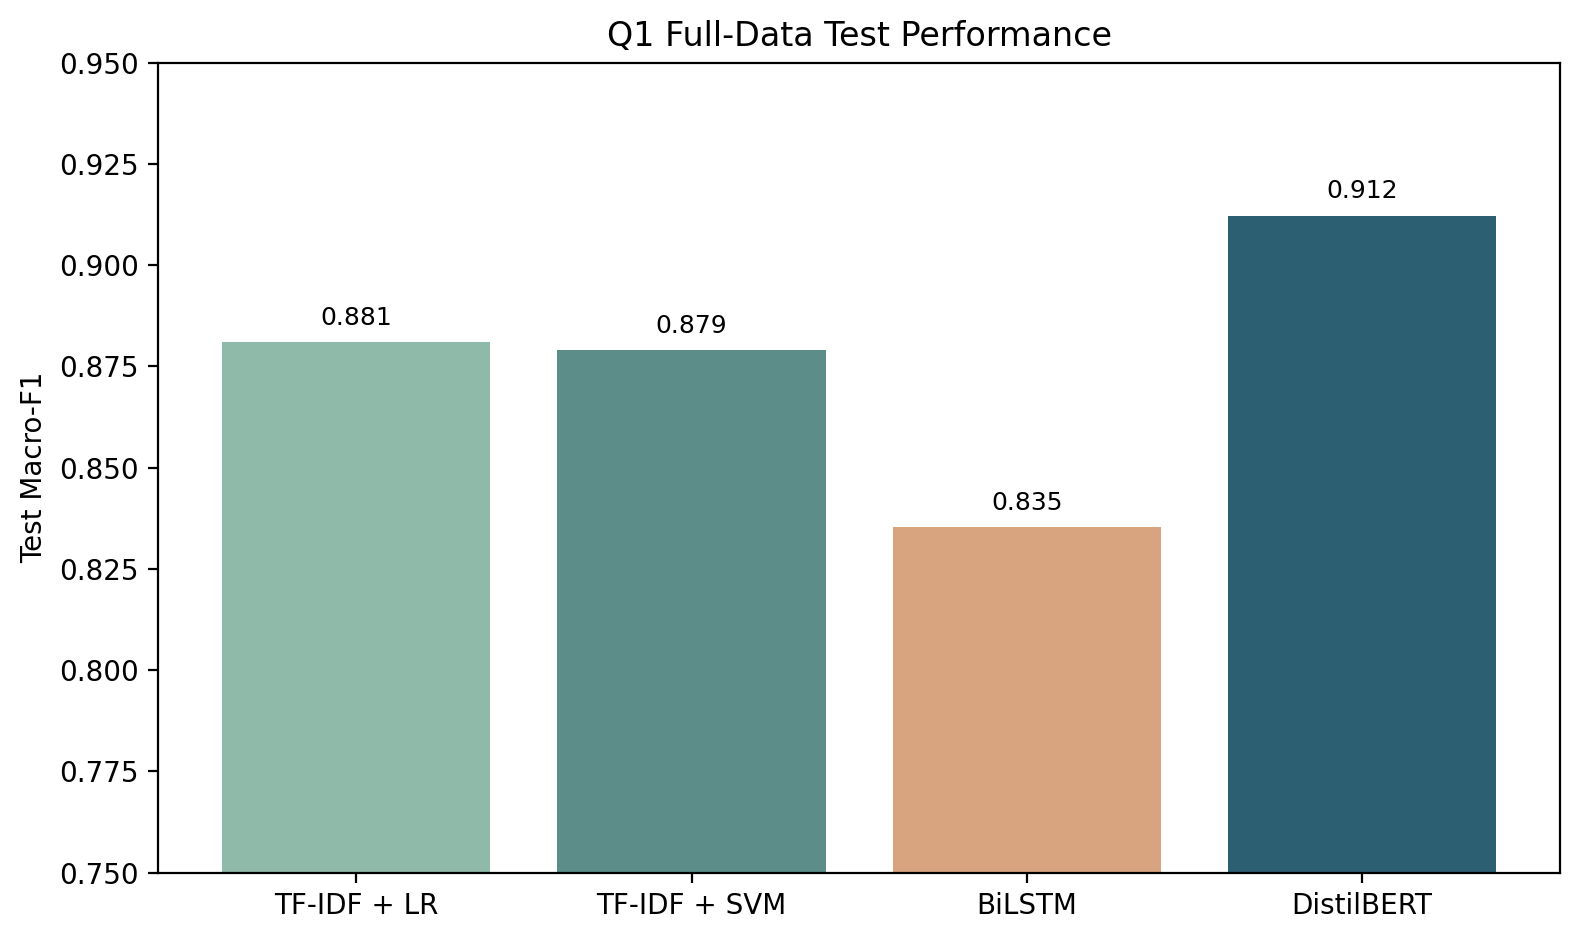
\includegraphics[width=0.85\textwidth]{figures/q1/model_comparison.png}
	\caption{Q1 full-data test macro-F1 comparison across TF-IDF, BiLSTM, and DistilBERT models.}
	\label{fig:q1_model_comparison}
\end{figure}

The neural runs now persist per-epoch histories, which makes convergence behavior explicit rather than implicit. Figure~\ref{fig:q1_distilbert_training_curve} shows that DistilBERT reaches its best validation macro-F1 by epoch 2 and then changes only marginally afterward, which is consistent with a stable fine-tuning regime rather than noisy late-epoch overfitting. On the test split, the same model remains balanced across both classes, with negative-review recall 0.9092 and positive-review recall 0.9153.

\begin{figure}[H]
	\centering
	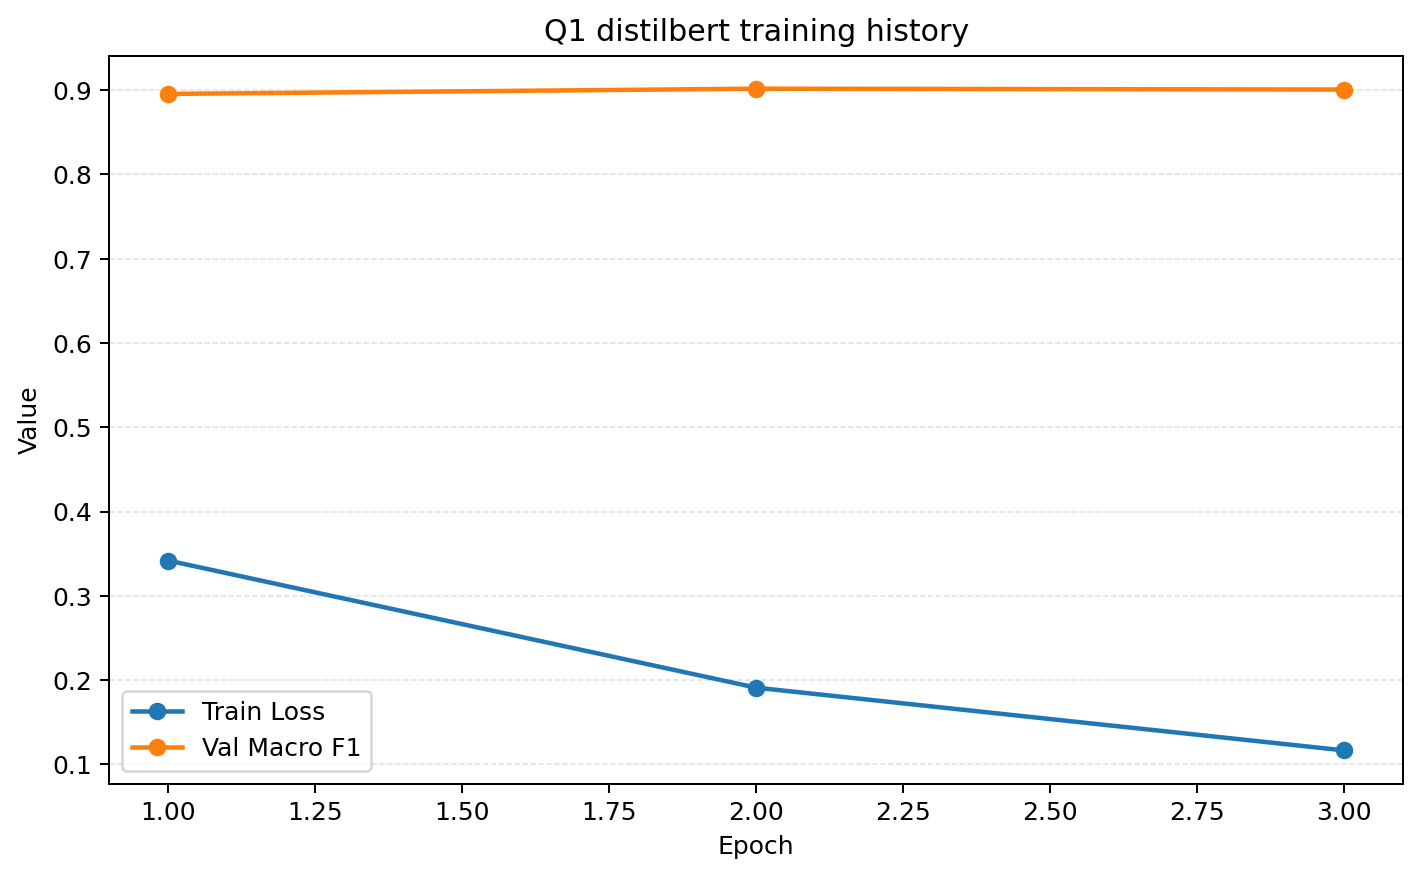
\includegraphics[width=0.78\textwidth]{figures/q1/distilbert_training_curve.png}
	\caption{Per-epoch training loss and validation macro-F1 for the full-data DistilBERT run.}
	\label{fig:q1_distilbert_training_curve}
\end{figure}

\subsection{Error Analysis}

The exported misclassification artifacts indicate that negation remains the dominant failure mode across all representation families. For both DistilBERT and the two TF-IDF baselines, 4 of the top 5 sampled test errors still fall into the \texttt{negation\_handling} category. The sparse models also show occasional mixed-sentiment and domain-specific ambiguity cases. BiLSTM is the most brittle model: in addition to negation, its sampled errors include very long reviews and broader discourse drift, which is consistent with a supervised-only sequence encoder that never closes the gap to the pretrained transformer.

This qualitative pattern matches the aggregate metrics. DistilBERT's contextual encoder is better at following sentiment reversals across long documents, TF-IDF remains surprisingly robust when the signal is lexical and local, and the supervised-only BiLSTM does not learn a representation strong enough to close the gap. In practical terms, the main unresolved Q1 errors are no longer simple vocabulary misses but cases where polarity depends on clause interaction, contrast, or delayed sentiment cues.

\subsection{Discussion}

The final full-data ranking for Question 1 is clear: DistilBERT is the strongest model, TF-IDF + Logistic Regression and TF-IDF + SVM remain strong lightweight baselines, and BiLSTM is the weakest of the finished runs. The most important takeaway is that representation choice matters more than small preprocessing differences on this task. The preprocessing sweep changed validation macro-F1 only marginally, whereas moving from sparse lexical features to contextual transformer embeddings produced the largest reliable gain.

At the same time, the results do not support a naive ``neural is always better'' conclusion. Moving from sparse features to a randomly initialized word-level BiLSTM still hurts performance, even after scaling the run to the full IMDb split. This makes the comparison more informative: the benefit comes from contextual pretraining rather than from replacing linear classifiers with a neural sequence model by itself. For the final report claim, DistilBERT should be presented as the best-performing Q1 model, TF-IDF as a strong and efficient baseline family, and BiLSTM as evidence that dense representations without pretraining are not sufficient on their own.